\documentclass[14pt]{extarticle} 
\usepackage{amsmath,mathtools,amsfonts,amsthm,amssymb,hyperref}
\usepackage{wasysym,geometry,bussproofs,latexsym,parskip,bookmark}
\usepackage{mathtools,float}
\newtheorem{defn}{Definition}
\newtheorem{thm}{Theorem}
\newtheorem{claim}{Claim}
\newtheorem{lemma}{Lemma}
\newcommand{\dps}{\displaystyle}
\hypersetup{colorlinks,allcolors=blue,linktoc=all}
\geometry{a4paper} 
\geometry{margin=0.5in}
\title{Math for CS 2015/2019 solutions to ``In-Class Problems Week 12, Wed. (Session 29)''}
\author{https://github.com/spamegg1}
\begin{document}
\maketitle
\tableofcontents

\section{Problem 1}
There is an unpleasant degenerative disease called Beaver Fever which causes people to tell unrelenting math jokes in social settings, believing other people would think they’re funny. Fortunately, Beaver Fever is rare, afflicting only about 1 in 1000 people. Doctor Meyer has a fairly reliable diagnostic test to determine who is going to suffer from this disease:

If a person will suffer from Beaver Fever, the probability that Dr. Meyer diagnoses this is 0.99.

If a person will not suffer from Beaver Fever, the probability that Dr. Meyer diagnoses this is 0.97.

Let $B$ be the event that a randomly chosen person will suffer Beaver Fever, and $Y$ be the event that Dr. Meyer’s diagnosis is “Yes, this person will suffer from Beaver Fever,” with $\overline{B}$ and $\overline{Y}$ being the complements of these events.

\subsection{(a)}
The description above explicitly gives the values of the following quantities. What are their values?

Pr[$B$] \,\,\,\,\,\, Pr[$Y | B$] \,\,\,\,\,\, Pr[$\overline{Y} | \overline{B}$]
\begin{proof}
Pr[$B$] = 1/1000, Pr[$Y | B$] = 0.99, Pr[$\overline{Y} | \overline{B}$] = 0.03
\end{proof}

\subsection{(b)}
Write formulas for Pr[$\overline{B}$] and Pr[$Y | \overline{B}$] solely in terms of the explicitly given quantities in part (a) - literally use their expressions, not their numeric values.
\begin{proof}
Pr[$\overline{B}$] = 1 - Pr[$B$], Pr[$Y | \overline{B}$] = 1 - Pr[$\overline{Y} | \overline{B}$]
\end{proof}

\subsection{(c)}
Write a formula for the probability that Dr. Meyer says a person will suffer from Beaver Fever solely in terms of Pr[$B$], Pr[$\overline{B}$], Pr[$Y | B$] and Pr[$Y | \overline{B}$].
\begin{proof}
Pr[$Y$] = Pr[$B$] $\cdot$ Pr[$Y|B$] + Pr[$\overline{B}$] $\cdot$ Pr[$Y|\overline{B}$]
\end{proof}

\subsection{(d)}
Write a formula solely in terms of the expressions given in part (a) for the probability that a person will suffer Beaver Fever given that Doctor Meyer says they will. Then calculate the numerical value of the formula.
\begin{proof}
By Bayes' Theorem

$$
Pr[B|Y] = \frac{Pr[Y|B]\cdot Pr[B]}{Pr[Y]}
$$

However Pr[$Y$] is not an expression given in part (a). So we need to use part (c) to replace it:

$$
Pr[B|Y] = \frac{Pr[Y|B]\cdot Pr[B]}{Pr[B] \cdot Pr[Y|B] + Pr[\overline{B}] \cdot Pr[Y|\overline{B}]}
$$

Now Pr[$\overline{B}$] and Pr[$Y|\overline{B}$] are not expressions given in part (a), so we need to use part (b) to replace them:

$$
Pr[B|Y] = \frac{Pr[Y|B]\cdot Pr[B]}{Pr[B] \cdot Pr[Y|B] + (1-Pr[B]) \cdot (1- Pr[\overline{Y}|\overline{B}])}
$$

Numerical value is

$$
Pr[B|Y] = \frac{0.99\cdot 0.001}{0.001 \cdot 0.99 + (1-0.001) \cdot (1- 0.03)} = 0.001020598
$$
\end{proof}

Suppose there was a vaccine to prevent Beaver Fever, but the vaccine was expensive or slightly risky itself. If you were sure you were going to suffer from Beaver Fever, getting vaccinated would be worthwhile, but by part (d), even if Dr. Meyer diagnosed you as a future sufferer of Beaver Fever, the probability you actually
will suffer Beaver Fever remains low (less than 1/30).

In this case, you might sensibly decide not to be vaccinated (after all, Beaver Fever is not that bad an affliction). So the diagnostic test serves no purpose in your case - you may as well not have bothered to get diagnosed. Even so, the test may be useful:

\subsection{(e)}
Suppose Dr. Meyer had enough vaccine to treat 2\% of the population. If he randomly chose people to vaccinate, he could expect to vaccinate only 2\% of the people who needed it. But by testing everyone and only vaccinating those diagnosed as future sufferers, he can expect to vaccinate a much larger fraction people who were going to suffer from Beaver Fever. Estimate this fraction.
\begin{proof}
If we calculate the numerical value of Pr[$Y$] from part (c) we get 0.03096 which means roughly 3\% of the population will be tested as future sufferers. Since Dr Meyer has enough vaccine for 2\% of the population, he can vaccinate 2/3 = 66\% of people who needed it.
\end{proof}

\section{Problem 2}
There are three prisoners in a maximum-security prison for fictional villains: the Evil Wizard Voldemort, the Dark Lord Sauron, and Little Bunny Foo-Foo. The parole board has declared that it will release two of the three, chosen uniformly at random, but has not yet released their names. Naturally, Sauron figures that he will be released to his home in Mordor, where the shadows lie, with probability 2/3.

A guard offers to tell Sauron the name of one of the other prisoners who will be released (either Voldemort or Foo-Foo). If the guard has a choice of naming either Voldemort or Foo-Foo (because both are to be released), he names one of the two with equal probability.

Sauron knows the guard to be a truthful fellow. However, Sauron declines this offer. He reasons that knowing what the guards says will reduce his chances, so he is better off not knowing. For example, if the guard says, “Little Bunny Foo-Foo will be released”, then his own probability of release will drop to 1/2 because he will then know that either he or Voldemort will also be released, and these two events are equally likely.

Dark Lord Sauron has made a typical mistake when reasoning about conditional probability. Using a tree diagram and the four-step method, explain his mistake. What is the probability that Sauron is released given that the guard says Foo-Foo is released?

Hint: Define the events S, F, and “F” as follows:

“F” = Guard says Foo-Foo is released

F = Foo-Foo is released

S = Sauron is released

\begin{proof}
In order to understand Sauron's error, let’s begin by working out the sample space, noting events of interest, and computing outcome probabilities:

\begin{figure}[ht!]
\centering
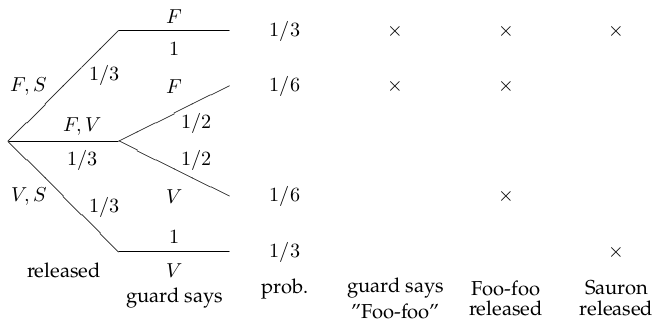
\includegraphics[scale=0.5]{sauron.png}
\end{figure}

The outcomes in each of these events are noted in the tree diagram.

Sauron’s error is in failing to realize that the event F (Foo-foo will be released) is different from the event “F ” (the guard says Foo-foo will be released). In particular, the probability that Sauron is released, given that Foo-foo is released, is indeed 1/2:

$$
\begin{array}{rcl}
Pr[S|F] & = & \dps\frac{Pr[S \cap F]}{Pr[F]}\\
& = & \dps\frac{1/3}{(1/3)+(1/6)+(1/6)}\\
& = & \dps\frac{1}{2}\\
\end{array}
$$

But the probability that Sauron is released given that the guard merely says so is still 2/3:

$$
\begin{array}{rcl}
Pr[S| ``F''] & = & \dps\frac{Pr[S \cap ``F'']}{Pr[ ``F'']}\\
& = & \dps\frac{1/3}{(1/3)+(1/6)}\\
& = & \dps\frac{2}{3}\\
\end{array}
$$

So Sauron’s probability of release is actually unchanged by the guard’s statement.
\end{proof}

\section{Problem 3}
There are two decks of cards. One is complete, but the other is missing the Ace of spades. Suppose you pick one of the two decks with equal probability and then select a card from that deck uniformly at random.

What is the probability that you picked the complete deck, given that you selected the eight of hearts? Use the four-step method and a tree diagram.

\begin{proof}
Let $C$ be the event that you pick the complete deck, and let $H$ be the event that you select the eight of hearts. In these terms, our aim is to compute:
$$
Pr[C|H] = \frac{Pr[C \cap H]}{Pr[H]}
$$
A tree diagram is worked out below:

\begin{figure}[ht!]
\centering
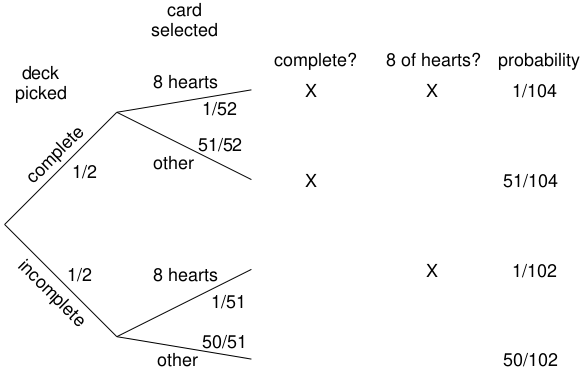
\includegraphics[scale=0.5]{two-decks.png}
\end{figure}

Now we can compute the desired conditional probability as follows:
$$
\begin{array}{rcl}
Pr[C|H] & = & \dps\frac{Pr[C \cap H]}{Pr[H]}\\
& = & \dps\frac{(1/2)\cdot(1/52)}{(1/2)\cdot(1/52) + (1/2)\cdot(1/51)}\\
& = & \dps\frac{51}{103}\\
& = & 0.498146\ldots\\
\end{array}
$$
Thus, if you selected the eight of hearts, then the deck you picked is less likely to be the complete one. It’s worth thinking about how you might have arrived at this final conclusion without going
through the detailed calculation.
\end{proof}

\section{Problem 4 (Supplemental Problem)}
Suppose you repeatedly flip a fair coin until you see the sequence HTT or HHT. What is the probability you see the sequence HTT first?

Hint: Try to find the probability that HHT comes before HTT conditioning on whether you first toss an H or a T. The answer is not 1/2.
\begin{proof}
Let's say that you win if we see HHT before HTT, I win if we see HTT before HHT.

This problem is tricky, because the game could go on for an arbitrarily long time. We will draw enough of the tree diagram to see a pattern, and then sum up the probabilities of the (infinitely many) outcomes in which you win.

It turns out that for any sequence of three flips, there is another sequence that is likely to come up before it. So there is no sequence of three flips which turns up earliest! . . . and given
any sequence of three flips, knowing how to pick another sequence that comes up sooner more than half the time gives you a nice chance to fool people gambling at a bar :-)

A partial tree diagram is shown below. All edge probabilities are 1/2.

\begin{figure}[ht!]
\centering
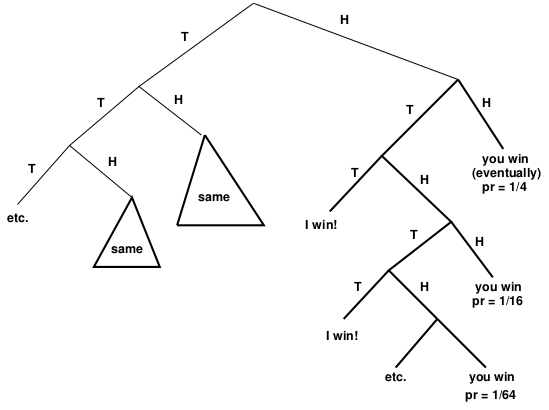
\includegraphics[scale=0.5]{htt.png}
\end{figure}

Let’s first focus on the subtree shown in bold (right half). Note that if two heads are flipped in a row, then you are guaranteed to win eventually. The sum of the probabilities of all your winning outcomes in this subtree is:

$$
\frac{1}{4} + \frac{1}{16} + \frac{1}{64} + \ldots = \frac{1}{4}\left(1 + \frac{1}{4} + \frac{1}{16} + \ldots \right) = \frac{1}{4} \cdot \frac{1}{1-(1/4)} = \frac{1}{3}
$$

The uppermost subtree marked same (middle) is identical to the one shown in bold (right half), except that each outcome probability is reduced by 1/2, because it is one edge farther from the root. Thus, the sum of your winning outcomes in this subtree is 1/6. Similarly, the next subtree marked same (bottom left) has each outcome probability reduced by 1/4 (because of the TT leading up to it), so the sum of your winning outcomes in that subtree is 1/12, and so forth. Overall, your probability of winning in the entire tree is:

$$
\frac{1}{3} + \frac{1}{6} + \frac{1}{12} + \ldots = \frac{1}{3}\left(1 + \frac{1}{2} + \frac{1}{4} + \ldots \right) = \frac{1}{3} \cdot \frac{1}{1-(1/2)} = \frac{2}{3}
$$

The probability of seeing HTT before HHT is the same as the probability that I win, which is 1/3.
\end{proof}

\end{document}
